\documentclass[ngerman]{scrartcl}
\usepackage[latin1]{inputenc}% erm\"oglich die direkte Eingabe der Umlaute 
\usepackage[T1]{fontenc} % das Trennen der Umlaute
\usepackage{ngerman} % hiermit werden deutsche Bezeichnungen genutzt und 
                     % die W\"orter werden anhand der neue Rechtschreibung 
		     % automatisch getrennt.
\usepackage[decimalsymbol=comma,
            loctolang={DE:ngerman,UK:english},
            separate-uncertainty = true,
            multi-part-units=single
            ]{siunitx}
\usepackage{paralist}
\usepackage{amsmath}
\usepackage{graphicx}
\usepackage{booktabs}
\usepackage{float}
\usepackage{caption}
\usepackage{subcaption}
\usepackage{tabularx}
\usepackage{array}
\usepackage{commath}
\usepackage{amsfonts}


\title{Praktikum Klassische Physik Teil 2 (P2)}
\subtitle{Interferenz}
\author{Simon Fromme, Philipp Laur}

\date{\today}

\begin{document}

%\parindent 0pt

\maketitle
\tableofcontents
\newpage

\section{Newonsche Ringe}
\subsection{Kr�mmungsradius einer bikonvexen Linse}
Um den Kr�mmungsradius zu bestimmen wurde der Aufbau der Vorbereitung gew�hlt. Mithilfe eines Fadenkreuzes, dass in dem Okular des Mikroskopes war konnten die Radien der einzelnen Minima bestimmt werden. Hierzu wurde die Linse mit dem beweglichen Objekttisch von Minima zu Minima bewegt. Um einen verl�sslichen Wert f�r den Radius zu erhalten (Fehler der Nullmessung), wird dies auf beiden Seiten gemacht.\\
Aus der Vorbereitung ist folgender linearer Zusammenhang bekannt:
\begin{align*}
r_K^2=\frac{R}{n_L}\cdot k\cdot \lambda
\end{align*}
F�r den weiteren Verlauf wird $n_L=1$ angenommen.\\
Gemessen wurde die gelbe und rote LED, hiereaus wurde Abb.1 (OriginPro 8.6G) erstellt.
\begin{figure}[h!]
\centering

	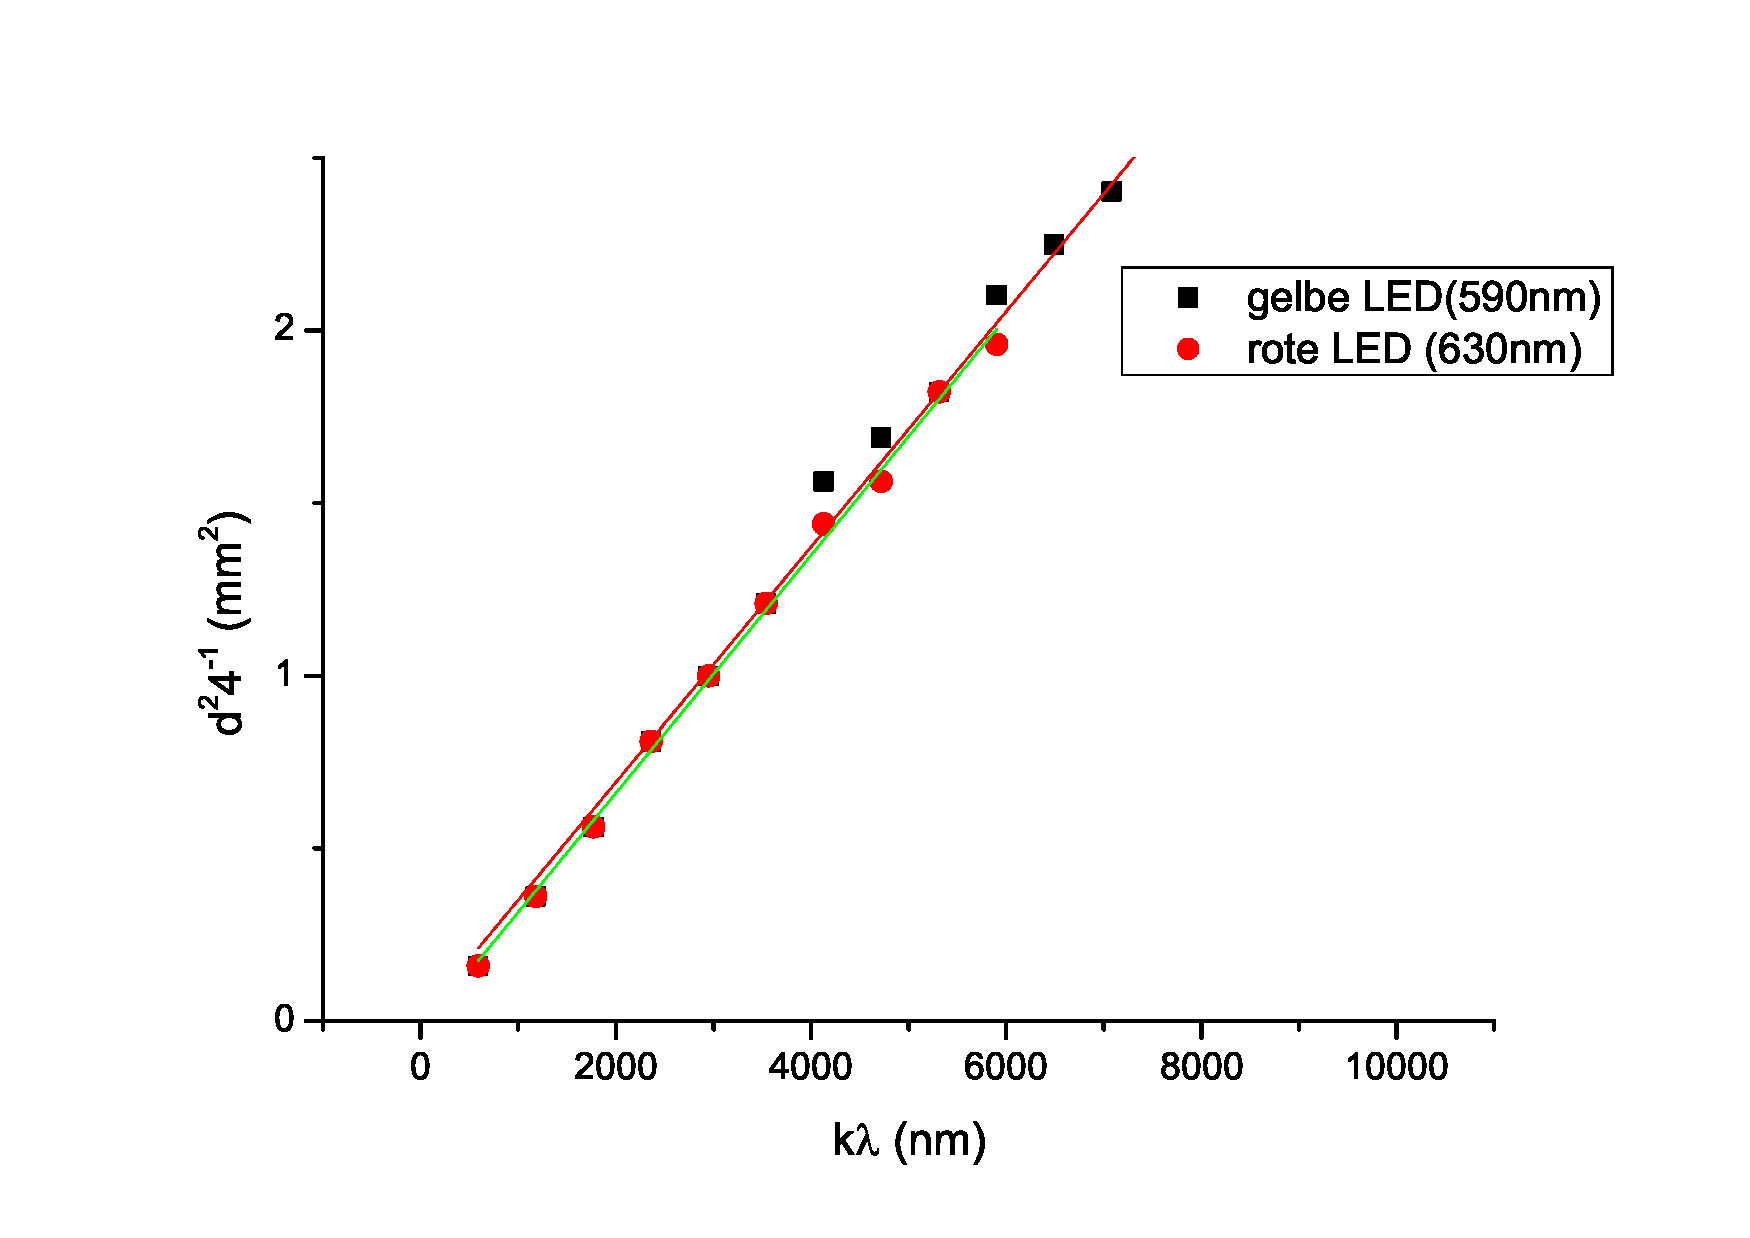
\includegraphics[scale=0.5]{Diagramme/1_1.eps}

\caption{Radien der Newtonschen Ringe f�r gelbes und rotes Licht}
\end{figure}
Die Steigung der Ausgleichsgeraden (hier: Werte f�r gelbe LED im weiteren Verlauf verwendet) ist unser gesuchter Kr�mmungsradius $R=\SI{34,096}{c\meter}$ (f�r die rote LED: $R_{rot}=\SI{34,445}{c\meter}$). Der statistische Fehler wurde mit Origin ermittelt, $\sigma_{R, stat}=\SI{0,007}{c\meter}$.\\
Der Fehler f�r die Messung des Radius wurde mit $\sigma_{r_K, sys}=\pm 0,05mm$ angenommen. Der Endwert entspricht dem Mittelwert der einzelnen Wertepaare.
\begin{align*}
\Delta R&=\left|\frac{\partial R}{\partial r_K}\right| \cdot \sigma_{r_K, sys}\\
&=\frac{2r_K}{k\lambda} \cdot \sigma_{r_K, sys}\\
&=\SI{1,552}{c\meter}\\
\Rightarrow R&=(34,096 \pm 0,007 \pm 1,552)cm
\end{align*}
\subsection{Brechungsindex von Wasser}
Nun wurden die Radien gemessen, w�hrend Wasser zwischen Linse und Objekttr�ger war. Dies erh�ht die Laufzeit zwischen diesen, wodurch es zu charakteristischen Werten kommt. Da der Kr�mmungsradius in Aufgabe 1.1 bestimmt wurde kann nun auf den Brechungsindex von Wasser geschlossen werden. Dies entspricht einer Auftragung von $r_{K, Luft}$ �ber $r_{K, Wasser}$, was in Abb. 2 gemacht wurde.
\begin{figure}[h!]
\centering

	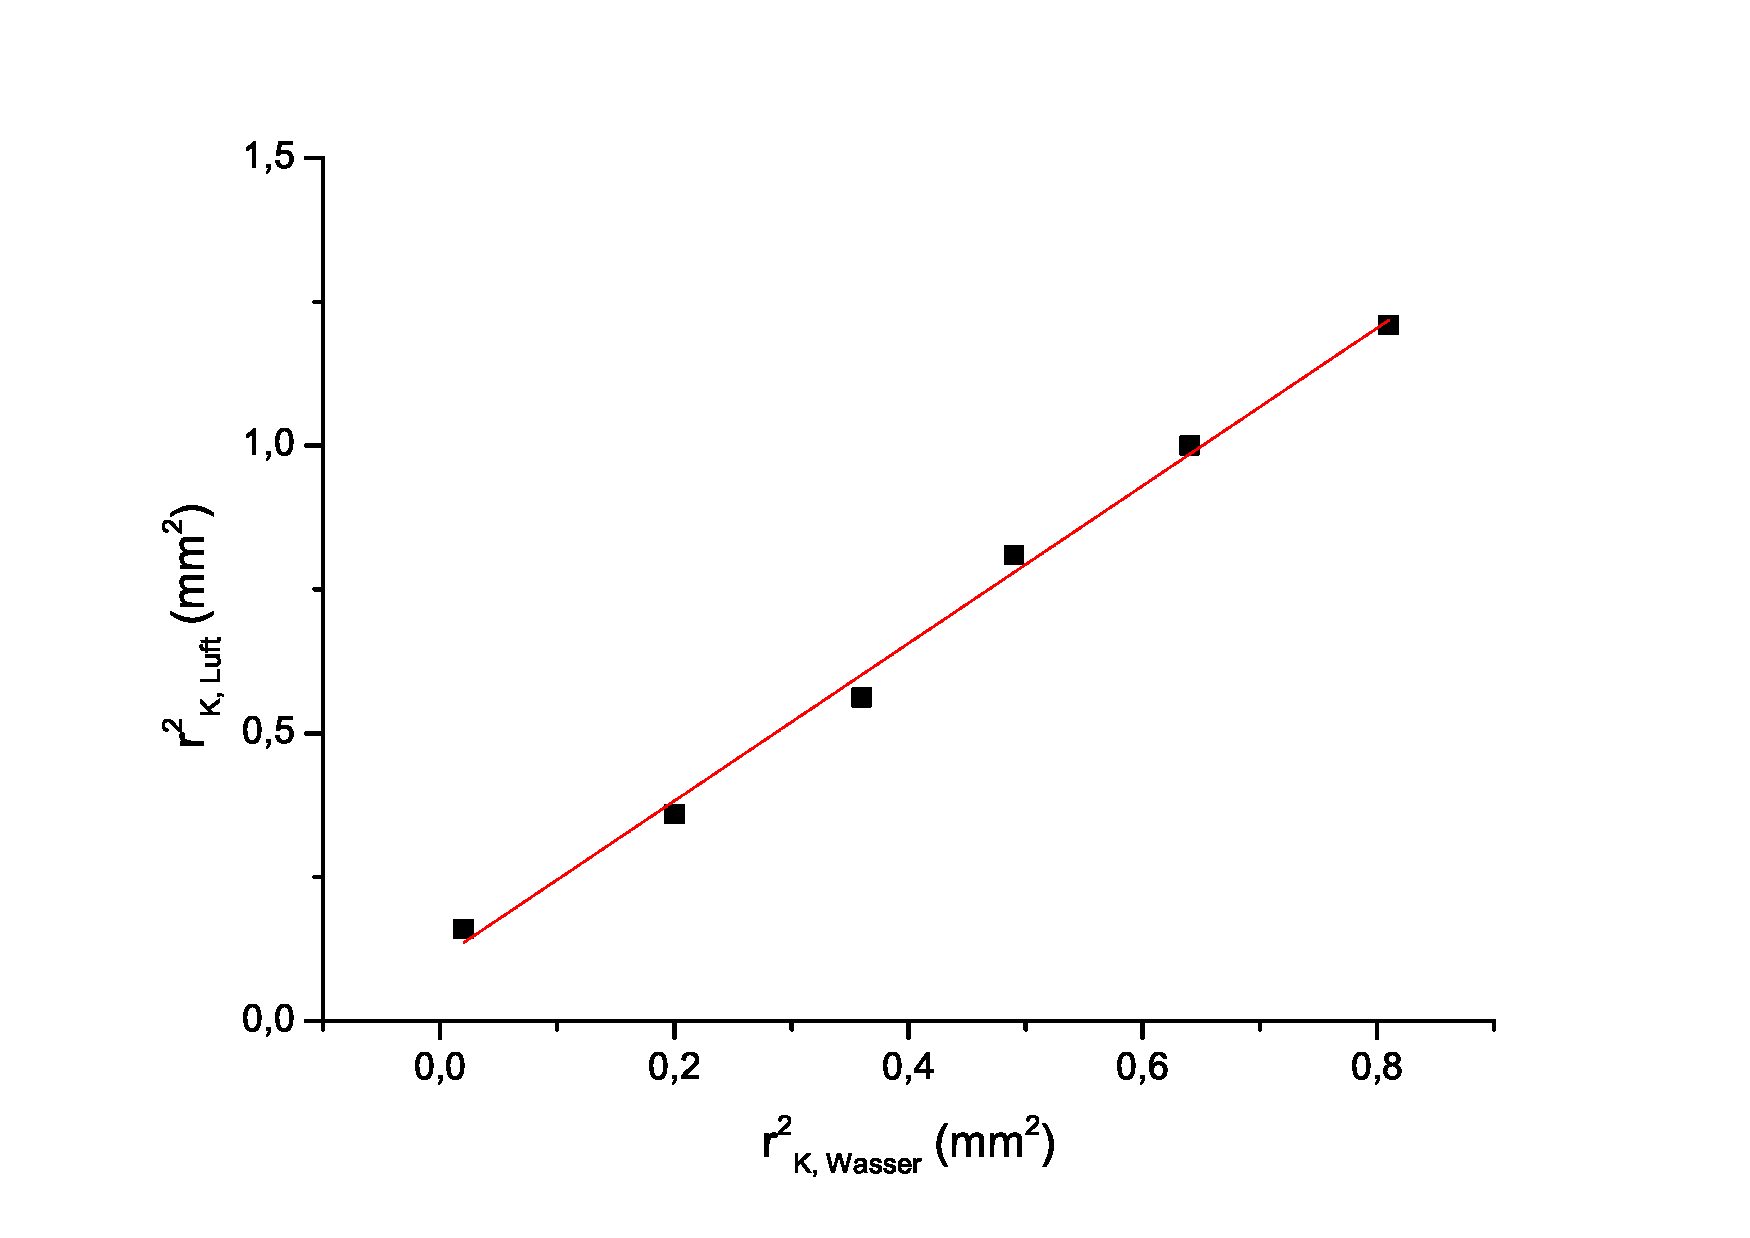
\includegraphics[scale=0.5]{Diagramme/1_2.eps}

\caption{Radien der Newtonschen Ringe ohne �ber mit Wasser (gelbes Licht)}
\end{figure}
Der Wert der Steigung ist unsere gesuchte Brechzahl:
\begin{align*}
n_{Wasser}=1,370 \pm 0,048
\end{align*}
Der Literaturwert liegt im Vertrauensbereich.
\subsection{Brennweite der Linse mittels Autokollimation}
Die Linse wurde so lange verschoben, bis der Gegenstand wieder scharf und spiegelverkehrt auf sich selbst abgebildet wird. Zu beachten gibt es, dass aufgrund der Reflexion Luft-Glas ein weiteres scharfes Bild vorhanden ist. Dieses darf aber nicht zur Bestimmung der Brennweite benutzt werden.\\
Im Gegensatz zur Vorbereitung muss der gemessene Wert halbiert werden, dies folgt aus der Linsengleichung. Aus den Messwerten ergibt sich der Mittelwert , sowie die Standardabweichung. Der systematische Fehler ergibt sich aus den Ablesefehlern, die wir mit insgesamt $\pm 0,6cm$ angenommen haben.
Hieraus ergibt sich f�r die Brennweite f der Linse:
\begin{align*}
f=(14,77 \pm 0,02 \pm 0,60)cm
\end{align*}
Der Wert liegt im Bereich der Angabe, die Linsen zwischen 5 und 35cm Brennweite vorhanden waren.
\subsection{Brechungsindex $n_{Glas}$ des Linsenglases}
F�r die bikonvexe Linse ergibt sich der Brechungsindex aus der Beziehung aus der Vorbereitung:
\begin{align*}
n_{Glas}&=\left( \frac{R}{2f}+1\right)\\
&=2,155
\end{align*}
Es k�nnte sich zum Beispiel um Zirkondioxid handeln.\\
Zur Bestimmung des statistischen Fehlers muss aufgrund der Korrelation mit R und f Gau�'sche Fehlerfortpflanzung angewandt werden:
\begin{align*}
\sigma_n &=\sqrt{\left(\frac{1}{2f}\right)^2 \sigma^2_R+\left(\frac{R}{2f^2}\right)^2 \sigma_f^2}\\
&=0,001
\end{align*}
Der systematische Fehler ergibt sich durch Gr��tfehlerabsch�tzung aus den beiden Gr��en zu:
\begin{align*}
\Delta n &= |\frac{1}{2f}|\cdot \Delta R+|\frac{R}{2f^2}|\cdot \Delta f\\
&=0,076\\
\Rightarrow n_{Glas}&=2,155 \pm 0,001 \pm 0,076
\end{align*}


\section{Beugung am Gitter}
\label{sec:beugung-am-gitter}

\subsection{Justierung des Gitterspektrometer}
\label{sec:just-des-gitt}

Alle Vorgaben zur Justierung und Scharfstellung des Gitterspektrometers werden der Aufgabenstellung entsprechend durchgef�hrt. Beachtenswert ist, dass die Scharfstellung durch Philipp Laur (normalsichtig), einige Ablesungen jedoch von Simon Fromme (leicht kurzsichtig) durchgef�hrt wurden. 

\subsection{Bestimmung der Gitterkonstante eines Gitters}
\label{sec:best-der-gitt}

In dieser Aufgabenstellung kam eine Natrium-Dampflampe zum Einsatz, deren mittlere Wellenl�nge $\lambda = \SI{589,3}{\nano\meter}$ bekannt ist. 

Im Versuch wurde die Winkel f�r die Maxima erster und zweiter Ordnung bestimmt, und jeweils die Winkeldifferenz $\Delta \alpha = \alpha_1 + (360� - \alpha_2)$ berechnent. Aus der Beziehung
\begin{align*}
  \lambda = \dfrac{N\cdot g}{\sin\left(\dfrac{\Delta \alpha}{2}\right)}
\end{align*}
ergibt sich die Gitterkonstante zu
\begin{align*}
  g = \dfrac{N\cdot\lambda}{\sin \left( \dfrac{\Delta\alpha}{2} \right)}
\end{align*}

Damit ergeben sich folgende Werte:
\begin{table}[htbp]
\centering
\caption{}
\begin{tabular}{rrrrr}
\toprule
$N$ & $\alpha_1$ in $\si{\degree}$ & $\alpha_2$ in $\si{\degree}$ & $\Delta\alpha$ in $\si{\degree}$ & $g$ in $\si{\nano\meter}$ \\ 
\midrule
1 & 21,083 & 339,083 & 42,000 & 1644,399 \\ 
2 & 45,667 & 314,300 & 45,683 & 1647,264 \\ 
\bottomrule
\end{tabular}
\label{}
\end{table}

Mittelt man �ber diese beiden Werte, so ergibt sich 
\begin{align*}
  g = \SI{1645,832}{\nano\meter}
\end{align*}

Mit einer abgesch�tzen Messunsicherheit beim Ablesen von $\alpha_1$ und $\alpha_2$ von $\Delta\alpha_1 = \Delta\alpha_2= '4 = \SI{0,066}{\degree}$ ergibt sich f�r den systematischen Fehler
\begin{align*}
  \Delta g_1 &= \left| \dpd{g_1}{\alpha_1} \right| \Delta\alpha_1 + \left| \dpd{g_1}{\alpha_2} \right| \Delta\alpha_2 \\
&= \dfrac{1}{2}\cdot N\lambda\cdot \dfrac{\cos \left( \dfrac{\Delta\alpha}{2} \right)}{\sin^2 \left( \dfrac{\Delta\alpha}{2} \right)} \left( \Delta\alpha_1 + \Delta\alpha_2 \right) \\
\end{align*}

Damit ergibt sich $\Delta g_1 = \SI{2,22}{\nano\meter}$ und $\Delta g_2 = \SI{3,19}{\nano\meter}$. Und damit der gesamte systematische Fehler zu: 

\begin{align*}
  \Delta g = \SI{2,70}{\nano\meter}
\end{align*}

Also
\begin{align*}
  g = (1645,83\pm 2,70) \si{\nano\meter}
\end{align*}


Die errechnete Gitterkonstante entspricht einer Liniendichte von $d = \SI{607,6}{\mm^{-1}}$, was dem angegebenen Wert von $d \approx \SI{600}{\mm^{-1}}$ sehr nahe kommt.

\subsection{Wellenl�ngenabstand der gelben Na-Linien}

Im Versuch konnte die Na-Doppellinie nur in der 2. Ordnung in zwei Linien unterschieden werden. Dort wurden bei einer Messung nach links und rechts jeweils folgende Unterschiede beobachtet:

\begin{table}[htbp]
\centering
\caption{Messergebnisse: Abstand Na-Doppellinie}
\begin{tabular}{lr}
\toprule
Messung nach & $\Delta\alpha$ in $\si{\degree}$ \\ 
\midrule
links & 0,100 \\ 
rechts & 0,067 \\ 
\bottomrule
\end{tabular}
\label{}
\end{table}



\subsection{Gitterkonstante eines zweiten Gitters.}
\label{sec:gitt-eines-zweit}

Mit Hilfe der vorliegenden Gitters k�nnen auch Maxima h�herer Ordnung bestimmt gemessen werden. In unserem Fall konnten diese bis zur Ordnung $N = 7$ abgelesen werden. Zur Bestimmung der Gitterkonstante eines zweiten Gitters verwendet man wie in der Vorbereitung gezeigt die Beziehung f�r Maxima
\begin{align*}
  N = g \dfrac{\sin \left( \dfrac{\Delta}{2} \right)}{\lambda}.
\end{align*}
Tr�gt man nun die Ordnung $N$ �ber $\sin \left( \frac{\Delta}{2} \right)$ auf, so ergibt sich die Gitterkonstante $g$ als Steigung der Regressionsgerade.

Man erh�lt mit $\lambda = \SI{589,3}{\nano\meter}$ und den Fehlerangaben von Gnuplot

\begin{align*}
  g = (6,16306\pm 0,0396) \si{\micro\meter}.
\end{align*}

Dies entspricht genau einer Strichst�rke von $d = \SI{162,2}{\mm^{-1}}$

% Anodenstrom - Thermokontaktspannung
\begin{figure}
  \centering
  \caption{Regression zur Bestimmung der Gitterkonstante}
  \input{Diagramme/gitterkonstante.tex}
\end{figure}



\subsection{Wellenl�ngen der Zn-Spektrallampe}
\label{sec:wellenlangen-der-zn}

Im letzten Versuchsteile werden die Wellenl�ngen des Spektrums einer Zn-Spektrallampe gemessen. Hierbei werden nur deutlich erkennbare Maxima abgelesen, da Schw�chere durch Verunreinigung des verwendeten Gases ebenfalls mit auftreten. 

Mit der Beziehung
\begin{align*}
  \lambda = \dfrac{g}{N}\cdot \sin \left( \dfrac{\Delta\alpha}{2} \right)
\end{align*}
wobei $\Delta\alpha$ der Winkelunterschied zwischen rechter und linker Messung ist, ergeben sich nach Mittlung �ber beide Ordnungen folgende Wellenl�ngen

\begin{table}[htbp]
\centering
\caption{Farben des Zn-Spektrums}
\begin{tabular}{rr}
\toprule
Farbe & $\lambda$ in $\si{\nano\meter}$ \\
\midrule
dunkelblau & 471,646 \\ 
blau & 475,326 \\ 
t�rkis & 484,513 \\ 
gr�n & 512,343 \\ 
rot & 641,639 \\ 
\bottomrule
\end{tabular}
\label{}
\end{table}



\end{document}